%\documentclass[10pt,letterpaper,twocolumn]{article}
\documentclass[10pt,letterpaper]{report}

%\usepackage{anysize}
%\marginsize{1in}{1in}{1in}{1in}
\usepackage{fullpage}

\usepackage{graphicx}

\hyphenpenalty=5000
\tolerance=1000

% Skip a line between paragraphs, and don't indent them
\setlength{\parskip}{10pt}  % 10 pt = space between paragraphs
\setlength{\parindent}{0pt} % 0 pt  = indentation

\begin{document}

\title{Photran 3.0 Developer's Guide}
\author{
% List of author names for the Photran developer's guide

J. Overbey \\
%your name here \\

}
\date{}

\maketitle

\tableofcontents

%%%%%%%%%%%%%%%%%%%%%%%%%%%%%%%%%%%%%%%%%%%%%%%%%%%%%%%%%%%%%%%%%%%%%%%%%%%%%%%

\chapter{Introduction}
% Introduction

Photran is a IDE for Fortran 90/95 and Fortran 77 that is built on top of
Eclipse.  It is structured as an Eclipse feature, in other words,
as a set of plug-ins that are designed to be used together.
Starting with version 3.0, it is an extension of CDT, the Eclipse IDE for
C/C++.  Previous versions of Photran were created by hacking a copy of the
CDT to support Fortran instead of C/C++, but now we have developed a
mechanism for adding new languages into the CDT, allowing the Fortran support
code to be in its own set of plug-ins.

Our purpose in writing Photran was to create a refactoring tool for Fotran.
Thus, Photran has a complete parser and program representation.  Photran
adds a Fortran editor and several preference pages to the CDT user interface,
as well as a Fortran Managed Make project type.

This document explains the design of Photran so that you could fix a bug or
add a refactoring.  You should know how to use Photran and how
the CDT works.  You need to understand Eclipse and Eclipse plug-ins
before you read this document.  We recommend \textit{The Java
Developer's Guide to Eclipse} for Eclipse newcomers.

\section{CDT Terminology}

The following are CDT terms that will be used extensively when discussing
Photran.

\begin{itemize}

\item \textbf{Standard Make projects} are ordinary Eclipse projects, except that
the CDT (and Photran) recognize them as being ``their'' type of project
(as opposed to, say, projects for JDT, EMF, or another Eclipse-based tool).
The user must supply their own Makefile, typically with targets ``clean''
and ``all.''  CDT/Photran cleans and builds the project by running
\texttt{make}.

\item \textbf{Managed Make projects} are similar to standard make projects,
except that CDT/Photran automatically generates a Makefile and edits
the Makefile automatically when source files are added to or removed
from the project.  The \textbf{Managed Build System} is the part of
CDT and Photran that handles all of this.

\item \textbf{Binary parsers} are able to detect whether a file is a legal
executable for a platform (and extract other information from it).
The CDT provides binary parsers for
Windows (PE), Linux (ELF), Mac OS X (Mach), and others.  Photran
does not provide any additional binary parsers.

\item \textbf{Error parsers} are provided for many compilers.  CDT provides
a gcc error parser, for example.  Photran provides error parsers for
Lahey Fortran, F, g95, and others.  Essentially, error parsers scan the
output of \texttt{make} for error messages for their associated compiler.
When they see an error message they can recognize, they extract the
filename, line number, and error message, and use it to populate the
Problems view.

\item CDT keeps a \textbf{model} of all of the files in a project.
The model is essentially a tree of \textbf{elements}, which all
derive from a (CDT Core) class \texttt{ICElement}.  It is described
in the next section.

\end{itemize}

\section{The Model}

The Make Projects view in Photran is essentially a visualization of
the CDT's \textit{model}, a tree data structure describing the contents
of all Make Projects in the workspace as well as the high-level contents
(functions, aggregate types, etc.) of source files.

Alain Magloire (CDT) described the model, A.K.A. the \texttt{ICElement}
hierarchy, in the thread
``Patch to create ICoreModel interface''
on the cdt-dev mailing list:

\begin{verbatim}
So I'll explain a little about the ICElement and what we get
out of it for C/C++.

The ICElement hierarchy can be separated in two:
(1) - how the Model views the world/resources (all classes above ITranslationUnit)
(2) - how the Model views the world/language (all classes below ITranslationUnit).

How we(C/C++) view the resources:
- ICModel  --> [root of the model]
    - ICProject --> [IProject with special attributes/natures]
        - ISourceRoot --> [Folder with a special attribute]
            - ITranslationUnit --> [IFile with special attributes, for example extensions *.c]
            - IBinary --> [IFile with special attributes, elf signature, coff etc...]
            - IArchive --> [IFile with special attributes, "<ar>" signature]
            - ICContainer -> [folder]

There are also some special helper classes
    - ILibraryReference [external files use in linking ex:libsocket.so, libm.a, ...]
    - IIncludeReference [external paths use in preprocessing i.e. /usr/include, ...]
    - IBinaryContainer [virtual containers regrouping all the binaries find in the project]

This model of the resources gives advantages:
- navigation of the binaries,
- navigation of the include files not part of the workspace (stdio.h, socket.h, etc ...)
- adding breakpoints
- search
- contribution on the objects
etc.....

[...]

(2) How we view the language.

Lets be clear this is only a simple/partial/incomplete view of the language.
For example, we do not drill down in blocks, there are no statements(if/else conditions) etc ....
For a complete interface/view of the language, clients should use the __AST__ interface.
\end{verbatim}

From another one of Alain's posts in that thread:

\begin{verbatim}
Lets make sure we are on the same length about the ICElement hierarchy.
It was created for a few reasons:

- To provide a simpler layer to the AST.  The AST interface is too complex
  to handle in most UI tasks.
- To provide objects for UI contributions/actions.
- The glue for the Working copies in the Editor(CEditor), IWorkingCopy class
- The interface for changed events.
- ...

Basically it was created for the UI needs: Outliner, Object action contributions,
C/C++ Project view and more.

The CoreModel uses information taken from:
- the Binary Parser(Elf, Coff, ..)
- the source Parser(AST parser)
- the IPathEntry classes
- the workspace resource tree
- The ResolverModel (*.c, *.cc extensions), ...

to build the hierarchy.
\end{verbatim}

\section{The CDT Debugger and \texttt{gdb}}

\begin{itemize}

\item The so-called CDT debugger is actually just a graphical interface to
\texttt{gdb}, or more specifically to \texttt{gdb/mi}.  If something
doesn't work, try it in \texttt{gdb} directly, or using another
\texttt{gdb}-based tool such as DDD.

\item The debugger UI ``contributes'' breakpoint markers and actions
to the editor.  The ``set breakpoint'' action, and the breakpoint markers
that appear in the ruler of the CDT (and Photran) editors are handled
entirely by the debug UI: You will \textit{not} find code for them in the
Photran UI plug-in.

\item \texttt{gdb} reads debug symbols from the executable it is debugging.
That is how it knows what line it's on, what file to open, etc.  Photran
has \textit{nothing} to do with this: These symbols are written entirely
by the compiler.  Moreover, the compiler determines what shows up in the
Variables view.  If the debugger views seem to be a mess, it is the
compiler's fault, not Photran's.

\end{itemize}


\chapter{Plug-in Decomposition}
% Plug-in Decomposition

Photran is actually a collection of several Eclipse plug-ins.
The following projects comprise Photran as it is distributed to users.

\begin{itemize}
\item{org.eclipse.photran.core

	This is the Photran Core plug-in.  It
	contains all of the ``behind the scenes'' functionality that
	supports Fortran-specific things in the user interface:
\begin{itemize}
	\item{IAdditionalLanguage for Fortran (i.e., the means
              of adding Fortran to the list of languages recognized
              by the CDT)}
	\item{Error parsers for Fortran compilers}
	\item{Fortran model builder and model elements}
	\item{Interface to Fortran parser (stored in f95parser.jar)}
	\item{Symbol table}
	\item{Module database (and Berkeley DB Java Edition)}
	\item{Refactorings, source printing, program manipulation}
	\item{Non-UI (parsing and model building) preferences}
\end{itemize}}

\item{org.eclipse.photran.managedbuilder.core, org.eclipse.photran.managedbuilder.ui

	This is the Managed Build system.
	Craig Rasmussen (LANL) is handling it.}

\item{org.eclipse.photran.cdtinterface

	This contains icons for all of the \texttt{FortranElement}s, i.e.,
	the icons used in the Outline and Make Projects views, and
	provides a method which returns \texttt{ImageDescriptor}s for them.}

\item{org.eclipse.photran.ui

	This contains the Fortran-specific components of the user interface:
\begin{itemize}
	\item{Editor}
	\item{Preference pages}
\end{itemize}}

\item{org.eclipse.photran-feature

	This is the Eclipse feature for Photran, used to build the Zip
	file distributed to users.  (A feature is a grouping of related
	plug-ins; in our case, all of the plug-ins listed above.)}

\end{itemize}

\noindent The following projects are in CVS but are not included directly in the
Photran distribution:

\begin{itemize}
\item{org.eclipse.photran-cdt-patches

	This contains CDT language extensibility/neutrality patches.}

\item{org.eclipse.photran-dev-docs

	This contains developer documentation, including this manual.}

\item{org.eclipse.photran-parser

	This contains the Fortran 95 parser, which is exported to
	f95parser.jar and stored in the Core plug-in.
	Note that this plug-in is not included directly in Photran
	and is not (should not be) referenced by any other plug-ins,
	since the parser is referenced through the JAR file
	(see parser description below).}

\item{org.eclipse.photran.tests

	This contains JUnit tests for the parser, symbol table builder,
	source printer, program editor, refactorings, etc.}

\item{org.eclipse.photran.xyzsamplelang

	This was my proof-of-concept for adding an additional language to
	the CDT.  It is completely independent of Photran.  It does
        not exist in the new Photran CVS repository and will soon be
        superceded by the Eightbol project.}

\end{itemize}


\chapter{CDT Integration}
% CDT Integration

Previous versions of Photran were developed by hacking the CDT: essentially,
we made the user interface say ``Fortran'' instead of ``C/C++,'' we replaced the
model builder (which creates the Outline view, among other things) with one
that ran a Fortran parser, we changed the list of file extensions, and we
modified the syntax highlighting code to recognize Fortran comments and
keywords.

Starting with Photran 3.0, we are taking a fundamentally different approach:
\begin{itemize}
\item We rename the C/C++ Perspective to the Make Perspective.  We replace
the four project types (C Standard Make Project, C++ Standard Make Project,
C Managed Make Project, and C++ Managed Make Project) with two generic
project types (Standard Make Project and Managed Make Project).  We also
change the launcher's menu item to read ``Run Local Application'' rather
than ``Run Local C Application.''  These are all superficial changes
(i.e., changes to labels and icons, not to the underlying code).  The
Make project types use the natures formerly used for C projects.
\item We add an extension point to the CDT which allows it to recognize
other languages besides C and C++.
\end{itemize}

\section{Integrating with the CDT: The \texttt{AdditionalLanguages}
            Extension Point}

The org.eclipse.photran.xyzsamplelang project is a simple example of how
to integrate a new language into the CDT.  Its README is included in an
appendix.

Essentially, the process of integrating a new language into the CDT works
as follows:
\begin{itemize}

\item Create a new plug-in with an editor.  (Obviously, you will eventually
want to customize the editor for your language.)

\item For each filename extension supported by your editor (i.e., each
filename extension for files in your language), declare a (text) content type.
\begin{verbatim}
   <extension point="org.eclipse.core.runtime.contentTypes">
      <content-type id="xyzSource" name="XYZ Language Source File"
            base-type="org.eclipse.core.runtime.text"
            priority="high"/>
      <file-association
            content-type="xyzSource"
            file-extensions="xyz"/>
   </extension>
\end{verbatim}

\item Specify org.eclipse.cdt.core as a dependency of your plug-in, and
declare in your \texttt{plugin.xml} that you are extending the
org.eclipse.cdt.core.AdditionalLanguages extension point.
\begin{verbatim}
   <extension point="org.eclipse.cdt.core.AdditionalLanguages">
      <language class="addl_langs.XYZLanguage"/>
   </extension>
\end{verbatim}
You must provide the fully-qualified name of a class
(\texttt{addl\_langs.XYZLanguage}, in this case which implements the
\texttt{org.eclipse.cdt.core.addl\_langs.IAdditionalLanguage} interface.

\item Fill in the definition of that class.  See the JavaDoc in
\texttt{IAdditionalLanguage} for more information.
\begin{itemize}
\item \texttt{getName} just returns the name of the language
(Fortran, XYZ Sample Language, etc.)
\item \texttt{getRegisteredContentTypeIds} returns a list of all of
the content types you declared above.  The content type names must
be fully qualified, i.e., the name of the plug-in followed by the name
of the content type, e.g., \texttt{XyzLanguagePlugIn.xyzSource}
or \texttt{org.eclipse.photran.core.fortranSource}.
\item \texttt{createModelBuilder} returns a model builder for your
language.  Look at the \texttt{ToyModelBuilder} in the XYZ Sample Language
project for a (trivial) example of how a model builder works, and
see the JavaDoc for \texttt{IModelBuilder} for a more complete description.
In essence,
\begin{itemize}
\item It must implement \texttt{IModelBuilder}.
\item Its constructor takes a \texttt{TranslationUnit}, i.e., the file
for which a model needs to be created.
\item The \texttt{parse} method return a Map taking
\texttt{ICElement}s to \texttt{CElementInfo}s, which contains all of the
elements that should appear in the Outline for the translation unit
specified in the constructor.  Use can either reuse the various implementations
of \texttt{ICElement} in the CDT (\texttt{Macro, Namespace,
FunctionDeclaration,} etc.), or you can create your own (with their own
icons) by implementing \texttt{IAdditionalLanguageElement}.
\end{itemize}
\end{itemize}

\item In the constructor for your editor, use the CDT UI plug-in's document
provider rather than your own, i.e.,
\begin{verbatim}
setDocumentProvider(CUIPlugin.getDefault().getDocumentProvider());
\end{verbatim}

\item Since you don't have your own document provider anymore, set up
your partitioner by overriding
\begin{verbatim}
protected void doSetInput(IEditorInput input)
\end{verbatim}
and setting it up there.

\item Reuse the Outline page provided by CDT by copying the following
field and methods from \texttt{FortranEditor} into
your editor (notice that we are passing \texttt{null} into the
constructor for \texttt{CEditorOutlinePage}; this doesn't seem to hurt
anything):
\begin{verbatim}
    protected CContentOutlinePage fOutlinePage;

    public Object getAdapter(Class required) { ... }

    public CContentOutlinePage getOutlinePage() { ... }

    public static void setOutlinePageInput(CContentOutlinePage page,
            IEditorInput input) { ... }
\end{verbatim}

\item If you want your editor to jump to the correct location when something
is selected in the Outline view, it needs to implement
\texttt{ISelectionChangedListener}.  (If you don't require this, remove
the line ``\texttt{fOutlinePage.addSelectionChangedListener(this);}''
from the code copied above.)  We implemented \texttt{ISelectionChangedListener}
by copying the following methods verbatim from \texttt{CEditor}:
\begin{verbatim}
    public void selectionChanged(SelectionChangedEvent event) { ... }

    private boolean isActivePart() { ... }

    public void setSelection(ISourceRange element, boolean moveCursor) { ... }
\end{verbatim}

\item If you want to be able to set breakpoints in your editor, add this
line to the constructor for your editor class:
\begin{verbatim}
    // JO: This gives you a "Toggle Breakpoint" action (and others)
    // when you right-click the Fortran editor's ruler
    setRulerContextMenuId("#CEditorRulerContext"); //$NON-NLS-1$
\end{verbatim}

\item If you want the CDT's Refactor menu to appear in your editor, add this
line to the constructor for your editor class:
\begin{verbatim}
    // JO: This will put the Refactor menu in the editor's
    // context menu, among other things
    setEditorContextMenuId("#CEditorContext"); //$NON-NLS-1$
\end{verbatim}

\end{itemize}

\section{Photran-CDT Integration}

Photran is integrated into the CDT in the same way described above.
\begin{itemize}

\item The Photran Core plug-in
defines a class \texttt{FortranLanguage}, which implements
\texttt{IAdditionalLanguage}, and hooks it into the (new)
\texttt{AdditionalLanguages} extension point in the CDT core.

\item Photran's Core plugin.xml defines a content type
\texttt{org.eclipse.photran.core.fortranSource}; \texttt{FortranLanguage}
notifies the CDT that we want it to treat this content type as a valid
source language.

\item We provide a \texttt{FortranModelBuilder}, which
runs our Fortran parser over a source file to create a CDT-compatible
model.

\begin{itemize}

\item Rather than using the CDT's model elements, we provide our own
model elements, which are all subclasses of \texttt{FortranElement}.
(\texttt{FortranElement} implements \texttt{IAdditionalLanguageElement}.)

\item The icons corresponding to \texttt{FortranElement}s
are stored in the org.eclipse.photran.modelicons plug-in.\footnote{
The Photran UI plug-in would be the logical place to store these icons.
However, the UI already has the Core as a dependency.  The icon requests
come from the \texttt{FortranElement}s in the Core, so if they had to be
retrieved from the UI, we would introduce a circular dependency.  So we put
them in their own plug-in.}

\end{itemize}

\item The Core plug-in also contributes several error parsers,
which are described in the next section.

\end{itemize}


\chapter{The Photran Core Plug-in}
% The Photran Core Plug-in

The Photran Core plug-in (org.eclipse.photran.core) contains several source
folders:

\begin{itemize}
\item \texttt{src} contains the main plug-in class
(\texttt{FortranCorePlugin}), the Fortran implementation of
\texttt{IAdditionalLanguage} (\texttt{FortranLanguage}), and any other
``miscellaneous'' classes that don't fit into one of the other folders.
\item \texttt{errorparsers} contains a number of built-in error parsers
for popular Fortran compilers.
\item \texttt{model} contains the model builder for Fortran
(\texttt{FortranModelBuilder}) and the Fortran model elements
(\texttt{FortranElement} and nested subclasses).
\item \texttt{parser} contains the \texttt{FortranProcessor} class,
which is an interface to the parser, which is stored in
\texttt{f95parser.jar}.  It also contains all of the symbol table classes.
\item \texttt{refactoring} contains everything related to refactoring
that is not used elsewhere in Photran, for example, the
\texttt{Program} and \texttt{Presentation} classes, the program editor,
the source printer, etc.  (All of these are described later.)
\item \texttt{preferences} contains classes which ``wrap'' the various
preferences that can be set in the Core plug-in.  The actual preference
pages displayed to the user are, of course, in the UI plug-in, but they
use these classes to get and set the preference values.
\end{itemize}

The parser JAR (\texttt{f95parser.jar}) is contained in the root folder
of this plug-in.

\section{Error Parsers}
Error parsers scan the output of \texttt{make} for error messages
for a particular compiler.
When they see an error message they can recognize, they extract the
filename, line number, and error message, and use it to populate the
Problems view.

For an example, see \texttt{IntelFortranErrorParser}.
(It's a mere 74 lines.)

To create a new error parser,
\begin{itemize}

\item In package \texttt{org.eclipse.photran.internal.errorparsers},
  define a class implementing \texttt{IErrorParser}

\item Implement \texttt{public boolean processLine(String line,
ErrorParserManager eoParser)}
  which should always returns false because ErrorParserManager appears not to
  use the result in a rational way

\item In org.eclipse.photran.core's \texttt{plugin.xml}, find the place
where we define all of the Fortran error parsers.  Basically, copy an
existing one.  Your addition will look something like this:
\begin{verbatim}
   <extension
         id="IntelFortranErrorParser"
         name="Photran Error Parser for Some New Fortran Compiler"
         point="org.eclipse.cdt.core.ErrorParser">
      <errorparser
            class="org.eclipse.photran.internal.errorparsers.MyErrorParser">
      </errorparser>
   </extension>
\end{verbatim}

\item Your new error parser will appear in the error parser list in the
Preferences automatically, and it will be automatically added to new projects.
For existing projects, you will need to open the project properties dialog
and add the new error parser to the project manually.

\end{itemize}

\textbf{Note.}  Error parsers to not have to be implemented in the Photran
Core plug-in.  In fact, they do not have to be implemented in Photran at all.
If you create a brand new plug-in, you can specify org.eclipse.cdt.core
as a dependency, include the above XML snippet in your plug-in's
\texttt{plugin.xml}, and include your custom error parser class in that
plug-in.


\chapter{The Photran UI Plug-in}
% The Photran UI Plug-in

The Photran UI plug-in (org.eclipse.photran.ui) contains the Fortran editor
and several preference pages.

Eclipse editors have a very non-intuitive structure which is very nicely
explained elsewhere (for example, in \textit{The Java Developer's Guide
to Eclipse}).

\section{Lexer-based Syntax Highlighting}

The main difference between our Fortran editor and a ``normal'' Eclipse
editor is that we do not use the typical means of syntax highlighting.
Since Fortran does not have reserved words, keywords such as ``if'' and
``do'' can also be used as identifiers.  So the word ``if'' may need
to be highlighted as a keyword in one case and as a varible in another.

To do this, we actually run the Fortran lexical analyzer over the entire
source file.  It splits the input into tokens and specifies whether they
are identifiers or not.  We create a partition for each token.  We also
create a partition for the space between tokens.  Each entire partition,
then, is given a single color, based on its contents (keyword, identifier,
or comments/whitespace).  This is all done in the class
\texttt{FortranPartitionScanner}.


\chapter{The Photran Lexers and Parser}
% The Photran Lexers and Parser

The Fortran 95 lexers and parser are stored in the org.eclipse.photran.parser
project.  Because this project takes several minutes and a lot of memory
(600-800 MB) to compile, it is exported as a (non-sealed) JAR archive,
\texttt{f95parser.jar}, which is stored in the Core plug-in.  The Core,
Managed Builder, and UI use classes from this JAR file, not from the
org.eclipse.photran.parser project.  So you do \textit{not} need the
org.eclipse.photran.parser project in your workspace unless you will be
regenerating this JAR file.

\section{Accessing the Lexers and Parser from Photran: The
         \texttt{FortranProcessor}}

(The following does \textit{not} apply to JUnit tests.)

To scan or parse a file, or to build a symbol table from a parse tree,
create a \texttt{FortranProcessor} and use it.  It knows how to distinguish
between fixed and free form file extensions based on the user's workspace
preferences and can determine whether or not parser debugging has been
enabled (also in the workspace preferences).

Examples:
\begin{itemize}
\item Parsing a file: See \texttt{FortranModelBuilder\#parse}
\item Lexing a file without parsing:
      See \texttt{FortranPartitionScanner\#documentChanged}
\item Creating a symbol table after a file has been parsed:
      (TODO-Jeff: No good examples yet)
\end{itemize}

\section{Structure of the Lexers and Parser}

Unfortunately, Fortran is not an easy language to process.  It has two
\textit{source forms,} and keywords are not reserved (so it's fine to call a
variable ``if'').  This greatly complicates lexical analysis.  To make
things as simple as possible, we have separated the lexical analysis into
several phases, depending on whether the input is in free form or fixed
form.

When a free form source file is being parsed...
\begin{itemize}

\item \texttt{FreeFormLexerPhase1}, which is generated from
\texttt{FreeFormLexerPhase1.flex} by JFlex, splits the input into tokens.
Tokens such as ``if,'' ``do,'' ``len=,'' etc. are labeled as keywords,
even if they are being used as identifiers (it doesn't know any better).

\item \texttt{FreeFormLexerPhase2} reads the token stream from
\texttt{FreeFormLexerPhase1} and buffers an entire statement worth of
tokens.  It then uses Sale's algorithm and an elaborate set of rules
(specified in the method \texttt{buildAdditionalRules}) to determine which
keyword tokens should be kept as keywords and which ones should actually
be identifiers.  In the case of ``keywords'' with an equal sign on the end
(such as ``len=''), if that token should really be an identifier, it is
split into two tokens: the identifier ``len'' and the = token T\_EQUALS.

\item The \texttt{Parser}, which is generated from \texttt{Fortran95.bnf}
by my parser generator, reads the tokens from \texttt{FreeFormLexerPhase2}
and parses the token stream, returning a parse tree.  The parse tree is
described in more detail later.

\end{itemize}

When a fixed form source file is being parsed...
\begin{itemize}

\item \texttt{FixedFormLexerPrepass} discards whitespace and comments
and concatenates continuation lines.

\item \texttt{FixedFormLexerPhase1}, which is generated from
\texttt{FreeFormLexerPhase1.flex} by JFlex, splits the input into tokens.
Essentially, it is identical to \texttt{FreeFormLexerPhase1}, except that
there are no rules for whitespace, comments, or line continuations.

\item \texttt{FreeFormLexerPhase2} reads the token stream from
\texttt{FixedFormLexerPhase1}, resolving identifiers as it does for free form
input.

\item \texttt{FixedFormLexerPhase2} reads the token stream from
\texttt{FreeFormLexerPhase2} and concatenates consecutive identifiers.

\item The \texttt{Parser} reads the tokens from \texttt{FixedFormLexerPhase2}.

\end{itemize}

\section{Parse Trees}

\subsection{Overview}
\textit{
\textbf{NOTE.}
We expect that you already know what a parse tree is and what the difference
is between abstract and concrete syntax.  Terms like ``terminal,''
``nonterminal,'' and ``token'' should be familiar.  If they are not,
you will need to spend some time with the Dragon book\footnote{Aho, Sethi,
and Ullman, \textit{Compilers: Principles, Techniques, and Tools}} before
tackling this section.}

When you call one of the \texttt{parse} methods on a \texttt{FortranProcessor},
either an exception will be thrown (if the lexer or parser encounters an
error), or the method will return a (non-null) parse tree.

A parse tree is just a tree of \texttt{ParseTreeNode}s with \texttt{Token}s
as leaves.  The \texttt{ParseTreeNode} returned by the \texttt{parse} method
is the root of the parse tree.

The parse tree for a program \textit{exactly} follows the derivation of the
program from the grammar in \texttt{Fortran95.bnf}.  It is literally a
parse tree, also known as a concrete syntax tree; it is \textit{not} an
abstract syntax tree (AST).\footnote{If you want to know why we didn't use an
abstract syntax tree, see the appendix on Miscellaneous Parser and Language
Processing Notes.} 

It is important to remember that the grammar in
\texttt{Fortran95.bnf} is different than the one in the Fortran standard.
The grammar in the Fortran standard is \textit{not} LALR(1)---not even
close---and so it had to be modified (quite heavily) to successfully
generate a parser from it.  So the parse trees you get from our parser are
\textit{not} always going to match what the Fortran standard grammar would
lead you to expect.  For example, there is no SFExpr in the Fortran standard
grammar, but you will find them popping up in your parse trees.

\textbf{TIP.}
When running Photran, go into your workspace preferences; in the Fortran Parser
section, there is an (very useful) option to ``display parse tree rather
than normal Outline view.''

\subsection{An Example}

\begin{figure}[h]
\centering
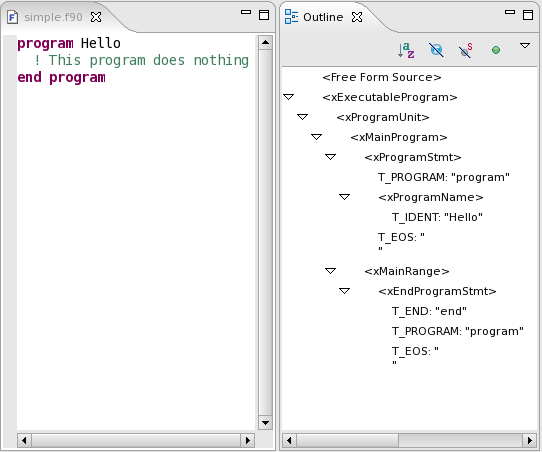
\includegraphics[width=5in]{images/parsetree1.png}
\caption{Sample program and its parse tree}
\label{parsetree}
\end{figure}

Figure \ref{parsetree} shows a trivial program and its parse tree.

\begin{itemize}

\item The node labels in angle brackets, such as $<$xExecutableProgram$>$ and
$<$xProgramStmt$>$, are nonterminals in the grammar and correspond to
\texttt{ParseTreeNodes} in the parse tree.\footnote{Note that $<$Free Form
Source$>$ (at the top of the Outline view) is just a label and not part of
the parse tree.}

\item Terminals in the grammar have names starting with T\_: for example,
T\_PROGRAM is the ``program'' keyword and T\_IDENT is an identifier.
Notice that the carriage return is also a token: end-of-statement (T\_EOS).
In the figure, these identify \texttt{Token}s in the parse
tree.\footnote{The distinction between terminals and tokens is somewhat
subtle.  Terminals are things like ``identifier,'' ``plus sign,'' and
``float'' that appear in a grammar.  Tokens are the actual chunks of text
from your input file, such as ``hello,'' ``+,'' and ``3.14.''  Every token
\textit{corresponds} to a terminal, e.g., ``hello'' is an identifier,
``+'' is (the only representation of) a plus sign, and ``3.14'' is a
float.}

\end{itemize}

Recall that each parse tree node corresponds to a nonterminal (on the
left-hand side of a production in the grammar) and each token corresponds
to a terminal.  

You can determine the nonterminal corresponding to a \texttt{ParseTreeNode}
by invoking \texttt{ParseTreeNode\#getRootNonterminal}.  (This method name
will soon be changed to \texttt{getCorrespondingNonterminal} or something
more intuitive like that.)  This will return a \texttt{Nonterminal}.  The
only valid \texttt{Nonterminal}s are all constants in the \texttt{Nonterminal}
class, so you can do identity comparisons like this:
\begin{verbatim}
if (parseTreeNode.getRootNonterminal() == Nonterminal.XEXECUTABLEPROGRAM) ...
\end{verbatim}

Similarly, you can determine the terminal corresponding to a token by
calling \texttt{Token\#getTerminal} and doing an identity comparison, as in
\begin{verbatim}
if (token.getTerminal() == Terminal.T_IDENT) ...
\end{verbatim}
You can get the text of the token (``Hello'' for the only T\_IDENT in
Figure \ref{parsetree}) by calling \texttt{Token\#getText}.

\texttt{Terminal}s and \texttt{Nonterminal}s both have a
\texttt{getDescription} method which returns a (String) description of that
terminal or nonterminal, e.g., ``T\_IDENT'' or ``$<$xExecutableProgram$>$.''


\chapter{Parse Tree Analysis: Visitors and Searching}
% Parse Tree Analysis

\textit{NOTE.  This section assumes that you are familiar with the Visitor
pattern\footnote{See Gamma, Helm, Johnson, and Vlissides, \textit{Design
Patterns}} and are familiar with symbol tables\footnote{See Aho, Sethi, and
Ullman, \textit{Compilers: Principles, Techniques, and Tools}}.}

\section{Visitors}

When you want to retrieve structural information about a program, typically
it will be done using a Visitor on the parse tree.

There are two types of Visitors available in Photran.
\begin{itemize}

\item A \texttt{ParseTreeVisitor} has a ``callback'' method for each nonterminal
in the grammar.  The tree is traversed in preorder, and as each node is visited,
a call is made to the Visitor method corresponding to the nonterminal for that node.
This is usually the preferred Visitor to use.

\item A \texttt{GenericParseTreeVisitor} only distinguishes between
\texttt{ParseTreeNode}s and \texttt{Token}s.  This Visitor should only be used
when all internal nodes are treated similarly.  If you need to distinguish between
the types of internal nodes, use a \texttt{ParseTreeVisitor} instead.

\end{itemize}

(\texttt{ParseTreeVisitor} is generated by the parser generator and should not
be modified.)

In addition to the visit methods, both types of Visitors have a
\texttt{preparingToVisitChildrenOf} method, which is called after a node has
been visited but before its children have, and a \texttt{doneVisitingChildrenOf}
method, which is called immediately after its children have been visited but
before any sibling nodes have.

\subsection{Creating and Using a Visitor}

Create a visitor by subclassing \texttt{ParseTreeVisitor} or
\texttt{GenericParseTreeVisitor}.  By default, all of the visit methods do
nothing, so you only have to override the methods that are useful to you.

Given the root of the parse tree (i.e., the \texttt{ParseTreeNode} returned
by \texttt{FortranProcessor\#parse}), use the \texttt{visitUsing} method
to traverse the parse tree; pass your visitor as the only argument.

\subsection{Sample Traversals}

As an example, consider again the ``do nothing'' program from Figure \ref{parsetree}.

When it is visited using a \texttt{GenericParseTreeVisitor}, the Visitor
methods are called in this order (methods called between \texttt{preparingToVisitChildrenOf}
and \texttt{doneVisitingChildrenOf} are indented to illustrate that child nodes
are being visited):

\begin{verbatim}
visitParseTreeNode(<xExecutableProgram>)
preparingToVisitChildrenOf(<xExecutableProgram>)
  visitParseTreeNode(<xProgramUnit>)
  preparingToVisitChildrenOf(<xProgramUnit>)
    visitParseTreeNode(<xMainProgram>)
    preparingToVisitChildrenOf(<xMainProgram>)
      visitParseTreeNode(<xProgramStmt>)
      preparingToVisitChildrenOf(<xProgramStmt>)
        visitToken(T_PROGRAM: "program")
        visitParseTreeNode(<xProgramName>)
        preparingToVisitChildrenOf(<xProgramName>)
          visitToken(T_IDENT: "Hello")
        doneVisitingChildrenOf(<xProgramName>)
        visitToken(T_EOS: (end of line))
      doneVisitingChildrenOf(<xProgramStmt>)
      visitParseTreeNode(<xMainRange>)
      preparingToVisitChildrenOf(<xMainRange>)
        visitParseTreeNode(<xEndProgramStmt>)
        preparingToVisitChildrenOf(<xEndProgramStmt>)
          visitToken(T_END: "end")
          visitToken(T_PROGRAM: "program")
          visitToken(T_EOS: (end of line))
        doneVisitingChildrenOf(<xEndProgramStmt>)
      doneVisitingChildrenOf(<xMainRange>)
    doneVisitingChildrenOf(<xMainProgram>)
  doneVisitingChildrenOf(<xProgramUnit>)
doneVisitingChildrenOf(<xExecutableProgram>)
\end{verbatim}

When it is visited using a \texttt{ParseTreeVisitor}, the Visitor
methods are called in this order:

\begin{verbatim}
visitXexecutableprogram(<xExecutableProgram>)
preparingToVisitChildrenOf(<xExecutableProgram>)
  visitXprogramunit(<xProgramUnit>)
  preparingToVisitChildrenOf(<xProgramUnit>)
    visitXmainprogram(<xMainProgram>)
    preparingToVisitChildrenOf(<xMainProgram>)
      visitXprogramstmt(<xProgramStmt>)
      preparingToVisitChildrenOf(<xProgramStmt>)
        visitXprogramname(<xProgramName>)
        preparingToVisitChildrenOf(<xProgramName>)
        doneVisitingChildrenOf(<xProgramName>)
      doneVisitingChildrenOf(<xProgramStmt>)
      visitXmainrange(<xMainRange>)
      preparingToVisitChildrenOf(<xMainRange>)
        visitXendprogramstmt(<xEndProgramStmt>)
        preparingToVisitChildrenOf(<xEndProgramStmt>)
        doneVisitingChildrenOf(<xEndProgramStmt>)
      doneVisitingChildrenOf(<xMainRange>)
    doneVisitingChildrenOf(<xMainProgram>)
  doneVisitingChildrenOf(<xProgramUnit>)
doneVisitingChildrenOf(<xExecutableProgram>)
\end{verbatim}

(The Visitors used to generate the output above are stored in
a JUnit test class called \texttt{ExampleVisitor}.)

\section{The \texttt{ParseTreeSearcher}}

Inside Visitor methods, typically you will want to look for particular tokens
or syntactic structures.

\subsection{An Example}

Consider the following (randomly selected) method from \texttt{DeclarationCollector},
one of the classes used for building symbol tables.
This class scans a program's parse tree, looking for declarations of programs, functions,
block data, namelists, etc., and inserts declarations for them into a symbol table.

\begin{verbatim}
    public void visitXmainprogram(ParseTreeNode node)
    {
        // # R1101 desn"t ensure ordering as the standard requires;
        // <xMainProgram> ::=
        //   <xMainRange> |
        //   <xProgramStmt> <xMainRange> ;
        // # R1102
        // <xProgramStmt> ::=
        //   <xLblDef> T_PROGRAM <xProgramName> T_EOS ;
        ParseTreeNode programStmt = ParseTreeSearcher.findFirstNodeIn(node, Nonterminal.XPROGRAMSTMT);
        Token name;
        if (programStmt != null)
	        name = ParseTreeSearcher.findFirstIdentifierIn(node);
        else
        {
	        name = new Token();
	        name.setText("(Anonymous Main Program)");
        }
        ...
\end{verbatim}

(The comment lines are copied from the parser generation grammar, \texttt{Fortran95.bnf}.)

In Fortran, a main program can either start with a program statement, or it
can not.  So both of these are valid programs:
\begin{verbatim}
program SayHi
  print *, 'Hello!'                             print *, 'Hello!'
end program SayHi                             end program SayHi
\end{verbatim}

In this Visitor method, \texttt{node} is guaranteed to be a $<$xMainProgram$>$,
due to the name of the method.  As shown, by looking at the grammar, we can
determine that it will either have one child (a \texttt{ParseTreeNode} corresponding
to an $<$xMainRange$>$) or two children (both \texttt{ParseTreeNode}s, the
first corresponding to an $<$xProgramStmt$>$ and the second corresponding to
an $<$xMainRange$>$.

If it \textit{does} have an $<$xProgramStmt$>$, then, a quick look at the rules for
$<$xLblDef$>$ (an optional integer label that can appear at the beginning of any
Fortran statement) and $<$xProgramName$>$ will make it evident that the first
identifier token (T\_IDENT) under the $<$xProgramStmt$>$ is the name of the program.

So now we can understand what this method does.
\begin{itemize}

\item It checks to see if the main program has a $<$xProgramStmt$>$.  This is done
by calling \texttt{ParseTreeSearcher\#findFirstNodeIn}, and telling it we want to
find the first $<$xProgramStmt$>$ that is a child of \texttt{node}.  It will either
return a \texttt{ParseTreeNode} corresponding to an $<$xProgramStmt$>$, or if it
can't find one, it will return \texttt{null}.

\item If there is an $<$xProgramStmt$>$, it grabs the first T\_IDENT token, which
tells the name the user gave to the program.

\item If there was no $<$xProgramStmt$>$, the program does not have a name, so we
``fake'' a token and name the program ``(Anonymous Main Program).''
\end{itemize}

\subsection{For More Information}

So, essentially, anytime you have a parse tree (or a subtree of the parse tree)
and you want to find a particular node or token, use one of the methods in
\texttt{ParseTreeSearcher}.  If there isn't one, you may have to write one yourself.
Be sure to look at the JavaDoc for the methods in that class; unless you are
doing something bizarre, one of the existing methods should work.


\chapter{Symbol Tables}
% Symbol Tables

All of the symbol table routines are stored in the ``parser'' folder under the
Core plug-in.

After you have parsed a file, you can create a symbol table for it by calling
\texttt{FortranProcessor\#createSymbolTableFromParseTree}.  This, in turn calls
the static method \texttt{SymbolTable\#createSymbolTableFor}, which is intended
to be the sole entrypoint for symbol table building.

\section{Contents of a Symbol Table}

The classes representing symbol table entries are stored in the
\texttt{org.eclipse.photran.internal.core.f95parser.symboltable.entries}
package.  Currently, the following are allowed.
\begin{itemize}
\item Main Programs
\item Modules
\item Functions
\item Subroutines
\item Derived Types
\item Block Data
\item Namelists
\item Common Blocks
\item Interfaces
\item Externals
\item Intrinsics
\item Variables
\end{itemize}

\texttt{FortranProcessor\#createSymbolTableFromParseTree} returns a
\texttt{SymbolTable}, which represents the global symbol table for
the program that was parsed.

A \texttt{SymbolTable} is essentially just a collection of
\texttt{SymbolTableEntry} objects.  Each \texttt{SymbolTableEntry} has
a child symbol table.  For \texttt{FunctionEntry} objects, this child
table contains all of the parameters, the return variable, and any
local variables declared inside the function.  For \texttt{VariableEntry}
objects, which represent local variables, the child table will always
be empty (it is there only for uniformity).

Symbol tables also keep track of whether an ``implicit'' rule applies,
what external modules are being used (via USE statements), etc.

To see what's in a symbol table, just use the \texttt{toString} method.
Child tables will be indented in the output.

The symbol table-related classes are JavaDoc'd, so additional information
is available there.

\section{\texttt{SymbolTableVisitor}s}

You can also create a Visitor for a program's symbol table hierarchy
by subclassing \texttt{SymbolTableVisitor}, which has a visit method
for each type of \texttt{SymbolTableEntry}.

\section{The Module Database}

Similar to \textit{import} statements in Java, Fortran programs can USE a
module defined in a different Fortran file.  Unfortunately, there is no
easy way to tell where this module might be defined.  The user simply specifies
a list of ``module paths'' which are searched for Fortran source files.
Each Fortran source file must be checked to see if it contains a module
with the given name.

In Photran, the list of modules paths is stored in a workspace preference,
although we plan to convert this to a project property.

The class \texttt{ModuleLoader} is responsible for locating modules in this
way.  The \texttt{ModuleDB} caches the symbol tables for files on the module
path so they don't all have to be reparsed every time a module is searched for.
Neither of these is complete yet, but they will be soon.

\section{How Symbol Tables are Built}

A quick look at \texttt{FortranProcessor\#createSymbolTableFromParseTree}
explains how symbol tables are built:
\begin{verbatim}
    public static SymbolTable createSymbolTableFor(ParseTreeNode parseTree) throws Exception
    {
        SymbolTable tbl = (new DeclarationCollector(parseTree)).getSymbolTable();
        Intrinsics.fill(tbl);
        return (new ReferenceCollector(tbl, parseTree)).getSymbolTable();
    }
\end{verbatim}

\begin{itemize}

\item A Visitor is run over the parse tree to collect declarations of
programs, modules, functions, subroutines, block data, derived types,
namelists, etc.---anything that can be stored in the symbol table.

\item The names of all Fortran 95 intrinsic functions and subroutines
are inserted into the table.

\item Now that declarations have been inserted, the parse tree is scanned
for references (i.e., uses of a function, variable, namelist, etc.).
If implicit variables have been allowed, the \texttt{ReferenceCollector} will
detect those (since they are used but not declared) and insert them into the
symbol table.

\end{itemize}


\chapter{Refactoring Support: Source Printing and Program Editing}
% Refactoring Support: Source Printing and Program Editing

Aside from the usual front end components (parser and symbol tables), a
refactoring tool requires
\begin{itemize}
\item a means of manipulating the parse tree, i.e., moving nodes around,
deleting them, and inserting new ones; and
\item a means of outputting ``revised'' source code after a parse tree has
been manipulated.
\end{itemize}

We will look at the means of outputting source code first, discussing
the \texttt{Presentation} and \texttt{SourcePrinter} classes.
We will then discuss the \texttt{ProgramEditor}, which allows you to
manipulate the parse tree and \texttt{Presentation}.

\section{The \texttt{Presentation} and the \texttt{Program}}

While the parse tree for a program stores all of the ``important'' tokens
(identifiers, parentheses, etc.), other things---comments, line continuations,
and C preprocessor directives---are not in the Fortran grammar.  However,
when the source printer produces source code from a parse tree, it needs to
include these as well.

We refer to these things (comments, line continuations, C preprocessor
directives, Fortran INCLUDE statements, and anything else that does not
end up in a parse tree) as \textit{non-tree tokens}, and we represent them
by the class \texttt{NonTreeToken}.  A \texttt{Presentation} is essentially
a list of all the non-tree tokens that appeared in a parse.

A \texttt{Presentation} can be created from a parse by calling the
\texttt{getNonTreeTokens} method on the lexer and passing the resulting
\texttt{List<NonTreeToken>} to the \texttt{Presentation} constructor.

A \texttt{Program} is just parse tree paired with a symbol table and a
\texttt{Presentation}.

\section{Presentation Blocks}

Since \texttt{Token}s in the parse tree and \texttt{NonTreeToken}s in
a program's \texttt{Presentation} have a lot in common, we will refer to
them collectively as ``presentation blocks.''  Not surprisingly, they
share a common superclass (interface, rather): \texttt{IPresentationBlock}.
JavaDoc removed, it looks like this:

\begin{verbatim}
public interface IPresentationBlock
{
    public abstract String getFilename();
    public abstract void setFilename(String value);

    public abstract int getStartLine();
    public abstract void setStartLine(int value);

    public abstract int getStartCol();
    public abstract void setStartCol(int value);

    public abstract int getEndLine();
    public abstract void setEndLine(int value);

    public abstract int getEndCol();
    public abstract void setEndCol(int value);

    public abstract int getOffset();
    public abstract void setOffset(int value);

    public abstract int getLength();
    public abstract void setLength(int value);

    public abstract String getText();
    public abstract void setText(String value);
}
\end{verbatim}

Intuitively, then, all presentation blocks know what file they originated from,
where they were in the file (both in terms of line/column and offset/length),
and exactly what their text looked like.  (This is important since capitalization
does not matter in Fortran.)

Most importantly, this means that reproduce the source code of a program verbatim
from a parse tree and a \texttt{Presentation}.  (The only difference will be the
use of spaces vs. tabs to make sure tokens appear in the correct column on a line.)
All comments and formatting will be retained.

\section{The \texttt{SourcePrinter}}

The job of the source printer (class \texttt{SourcePrinter}) is to take a
a parse tree and corresponding \texttt{Presentation}
and produce source code from it.

Since every \texttt{Token} in the parse tree and every \texttt{NonTreeToken}
in the \texttt{Presentation} knows what line and column it should appear on,
this is easy.

\section{The \texttt{ProgramEditor}}

Essentially, a refactoring needs to change the parse tree for a program.  It
may change existing nodes, move them around, remove them altogether, or insert
new nodes.

As described above, though, source code is produced by looking at the line/column
offsets of the \texttt{Token}s in the parse tree and interleaving comments and
other non-tree tokens from a program's \texttt{Presentation}.

When we add, move, change, or delete a subtree of the parse tree, then,
we must do three things:
\begin{itemize}
\item adjust the positions of the \texttt{Token}s in that subtree,
\item adjust the positions of the related \texttt{NonTreeToken}s
(e.g., the comments describing a method and C preprocessor directives in its
definition)
\item adjust the positions of all of the presentation blocks that appear after
the modified subtree.  For example, if you change an token's text from
``Hello'' to ``Goodbye,'' every presentation block after that one will have
its offset incremented by 2, and every presentation block to the right of
that token on the same line will also have its starting column number incremented
by 2.
\end{itemize}

The (static) methods in \texttt{ProgramEditor} are used to add, move, modify,
and delete subtrees.

This class will be described more as it stabilizes.


\chapter{Refactoring: Preconditions and Implementation}
% Refactoring: Preconditions and Implementation

From an implementation standpoint, a refactoring consists of
\begin{itemize}
\item a set of \textit{initial preconditions},
\item input from the user,
\item a set of \textit{final preconditions}, and
\item a program manipulation.
\end{itemize}

As an example, consider the easiest of all refactorings: Rename.
\begin{itemize}
\item \textbf{Initial preconditions:}
    \begin{itemize}
    \item The token to rename should be an identifier.
    \item The identifier must correspond to an entry in the symbol table.
    \item If Rename is limited to certain entities, say, variables and subprograms,
          the symbol table entry should indicate that the identifier corresponds
          to a variable or subprogram.
    \end{itemize}
\item \textbf{User input:}
    \begin{itemize}
    \item New name for the variable or subprogram
    \end{itemize}
\item \textbf{Final preconditions:}
    \begin{itemize}
    \item The new name must be a valid identifier.
    \item The new name must be different from the old name.
    \item The new name must not already exist in its namespace.
    \item For every reference to the old name, a change to the new name should uniquely
          identify the same variable or function.  For example, if you are renaming a
          global variable from \texttt{a} to \texttt{b}, but a local variable \texttt{b}
          will end up shadowing the global variable and cause one of its references to
          ``go wrong,'' then the rename cannot continue.
    \end{itemize}
\item \textbf{Program manipulation:}
    \begin{itemize}
    \item Locate the declaration of the entity being renamed, and locate all
          references in all files in the workspace, and change the token text
          to the new name.
    \end{itemize}
\end{itemize}

The distinction between initial and final preconditions, then, is that
initial preconditions must be satisfied before the user is asked for input,
while final preconditions depend on the user's input.  If a refactoring does
not require user input, it will have no final preconditions.

\section{Running a Refactoring}

Running a refactoring looks something like this.\footnote{The
\texttt{if (!...) throw ...} is an obvious code smell that makes it look like
the various methods in \texttt{RenameRefactoring} should be throwing exceptions
rather than returning booleans.  The current structure makes more sense in
``real'' code, where the user is being assaulted with dialog boxes and other
things happen between each of the steps.}

\begin{verbatim}
        RenameRefactoring r = new RenameRefactoring(getProgram(), targetToken);
        if (!r.checkInitialPreconditions()) throw new Error(r.getErrorMessage());
        r.setNewName("Whatever");
        if (!r.checkFinalPreconditions()) throw new Error(r.getErrorMessage());
        if (!r.perform()) throw new Error(r.getErrorMessage());
\end{verbatim}

In other words, you
\begin{itemize}
\item check the initial preconditions,
\item get input from the user,
\item check the final preconditions, and
\item finally perform the refactoring.
\end{itemize}
At any point, if a step has failed, you can call \texttt{r.getErrorMessage()}
to get an explanation suitable for displaying to the user.

\section{The \texttt{FortranRefactoring} Class}

All Fortran refactorings must be subclasses of \texttt{FortranRefactoring}.
\texttt{FortranRefactoring} (or its superclass) provides
\begin{itemize}
\item an instance variable \texttt{error}, the contents of which will be
      returned
      when the user calls \texttt{getErrorMessage()}.  If the refactoring fails,
      before returning false, be sure to set this so the user knows why.
\item Two \texttt{List}s of \texttt{Precondition}s:
      \texttt{initialPreconditions}
      and \texttt{finalPreconditions}.  Add preconditions to the former in the
      constructor and the latter after input has been received from the user.
\item Two fields, \texttt{initialPreconditionsCheckedAndPassed} and
      \texttt{finalPreconditionsCheckedAndPassed}.  For example, you will want
      to assert that the initial preconditions have been checked and passed
      before checking the final preconditions.
\end{itemize}

\section{Preconditions}

Refactoring preconditions are stored in the package
\texttt{org.eclipse.photran.internal.core.refactoring.preconditions}.
They are all derived from the class \texttt{AbstractPrecondition}.

A precondition (i.e., a class derived from \texttt{AbstractPrecondition})
has:
\begin{itemize}
\item a \texttt{List} of prerequisite preconditions, and
\item a method for checking this precondition.
\end{itemize}

To check a precondition, call its \texttt{check} method.  After this method
has been called once, it ``remembers'' whether it succeeded or failed, so
future calls to \texttt{check} will just return the stored result rather than
performing the entire check again.\footnote{It is very possible that a
precondition will be checked manually, and then it will be checked again
because it is a prerequisite for another precondition.  This resolves any
inefficiences that might result because of this.}

To implement how a precondition is checked, override the abstract method
\texttt{checkThisPrecondition} method.  If any other preconditions need
to be checked before this one, add them to the \texttt{prereqPreconditions}
list in the constructor.  If the code in \texttt{checkThisPrecondition} is
called, they have all been satisfied.

The fields \texttt{parseTree}, \texttt{presentation}, and \texttt{symbolTable}
will be populated when the constructor is called.  You will almost definitely
need to use these in your implementation of \texttt{checkThisPrecondition}.

\section{Implementing a Refactoring}

\begin{itemize}

\item If you need any preconditions that don't exist yet, implement them
      as described above.

\item Create a subclass of \texttt{FortranRefactoring}.

\item In the constructor, call \texttt{super} and add preconditions
      to the \texttt{initialPreconditions} field.

\item Implement any methods to store input from the user.  At the beginning
      of these methods, you will probably want to assert
      \texttt{initialPreconditionsCheckedAndPassed}.

\item Implement \texttt{perform}.  You will want to assert that all user
      input is in place as well as asserting
      \texttt{finalPreconditionsCheckedAndPassed}.  Use the
      \texttt{ProgramEditor} to modify the parse tree and presentation.
      If your changes might possibly affect the program's symbol table,
      call the (inherited) \texttt{rebuildSymbolTable} method after all
      transformations have been completed.

\end{itemize}

TODO-Jeff: Figure out and document how to integrate a refactoring into the
(CDT) UI.


%%%%%%%%%%%%%%%%%%%%%%%%%%%%%%%%%%%%%%%%%%%%%%%%%%%%%%%%%%%%%%%%%%%%%%%%%%%%%%%
\appendix

\chapter{Getting the Photran 3.0 Sources from CVS}
\vspace{0.5em}
% Getting the Photran 3.0 Sources from CVS

\hspace{1em}\textbf{Part I.  Check out the CDT sources from CVS}

\begin{enumerate}
\item  In Eclipse, switch to the CVS Repository Exploring perspective.
\item  Right-click the CVS Repositories view; choose New, Repository Location
\item  Enter the following information, then click Finish: \\
\begin{tabular}{ll}
         Host name:       & dev.eclipse.org \\
         Repository path: & /home/tools \\
         Connection type: & pserver \\
         Username:        & anonymous \\
         Password:        & (no password) \\
\end{tabular}
\item  Right-click on :pserver:anonymous@dev.eclipse.org:/home/tools, and choose
    Refresh Branches...
\item  Select the following, and click OK:
\begin{itemize}
    \item     org.eclipse.cdt-build
    \item     org.eclipse.cdt-core
    \item     org.eclipse.cdt-doc
    \item     org.eclipse.cdt-debug
    \item     org.eclipse.cdt-launch
\end{itemize}
    When prompted, tell it to Search Deeply.
\item  Expand :pserver:anonymous@dev.eclipse.org:/home/tools,
    and then expand Versions (in the CVS Repositories view)
\item  Under org.eclipse.cdt-build, expand org.eclipse.cdt-build CDT\_3\_0\_RC2
\item  Right click and check out all of the org.eclipse.cdt.* packages
    EXCEPT for the ones ending in "tests" (why bother testing?)
\item  Do the same with org.eclipse.cdt-core, org.eclipse.cdt-debug,
    org.eclipse.cdt-doc, and org.eclipse.cdt-launch
\item You now have the CDT source code.  Make sure it compiles successfully
    (lots of warnings, but no errors).

\vspace{.5em}
\noindent\textbf{Part II.  Check out the Photran source and the CDT patches}

\item In Eclipse, switch to the CVS Repository Exploring perspective.
\item Right-click the CVS Repositories view; choose New, Repository Location
\item Enter the following information, then click Finish: \\
\begin{tabular}{ll}
        Host name:       & www.photran.org \\
        Repository path: & /usr/local/photran30-new \\
        Connection type: & extssh \\
        Username/passwd: & (we gave you this) \\
\end{tabular}
\item Expand extssh:username@www.photran.org:/usr/local/photran30-new,
    then expand HEAD (in the CVS Repositories view)
\item{Right-click and check out all of the org.eclipse.photran projects EXCEPT
    org.eclipse.photran-parser.
    You only need this project if you will be regenerating the parser from the
    grammar.  (The parser is included in the org.eclipse.photran.core plug-in
    as a JAR file.  This way, the parser does not have to be recompiled
    every time you rebuild Photran.)}

The sources will NOT compile at this point; you must complete the following...

\vspace{.5em}
\noindent\textbf{Part III.  Patch the CDT sources}

\item Go to a bash prompt.  Change to your Eclipse workspace directory
    (the one containing all of the org.eclipse.cdt and
    org.eclipse.photran projects).
\item Change (\texttt{cd}) to the org.eclipse.photran-cdt-patches directory.
\item Run ./install
\item{Go back into Eclipse.  Refresh all of the org.eclipse.cdt packages.
    (Click the first, shift-click the last, right-click, choose Refresh.)}

The sources should all compile (albeit with about 640 warnings).
\end{enumerate}


\chapter{XYZ Language Plug-in README}
% XYZ Language Plug-in README

The org.eclipse.photran.xyzsamplelang project demonstrates
how to use the \texttt{AdditionalLanguages} extension point.
It is just the sample XML editor plug-in that gets created when you choose
to create a new plug-in project and select the ``plug-in with an editor''
template.  However, it has been modified to integrate with the CDT.
Here is the README from that project, which is a cursory description of
how the CDT was modified and how the XYZ language was integrated.  The
specific changes to the editor are documented in its code, so be sure
to read that too!

\begin{verbatim}
* * * * * * * * * * * * * * * * * * * * * * * * * * * * * * * * * * * * * * * *


   HOW TO TIE A NEW SOURCE FILE TYPE, PARSER, AND MODEL BUILDER INTO THE CDT
                     (AND HOW TO MAKE THE CDT ALLOW IT)


* * * * * * * * * * * * * * * * * * * * * * * * * * * * * * * * * * * * * * * *

If you create your own editor, model builder, and ICElement-derived elements,
some simple changes to the CDT source code will make the CDT
integrate your parser and the elements it produces into its model.

We add an AdditionalLanguages extension point to the CDT Core and change a
couple of methods to make use of it.

* * * * * * * * * * * * * * * * * * * * * * * * * * * * * * * * * * * * * * * *

NOTE ON INCLUDED SOURCE CODE:

All files in the CDT Integration Proof-of-Concept - Phase 1 source folder were
generated by the New Plug-In wizard EXCEPT:

- Several changes were made to the editor's main class (XyzLanguageEditor) and
  are commented there
- I added FortranContentOutlinePage
- I added the ToyElement and ToyModelBuilder classes (based on Photran's
  FortranElement hierarchy and its (hidden) ToyModelBuilder)
- I added XyzLanguagePerspective, which gives us our own perspective and adds
  a shortcut for our new file wizard to the New File menu

* * * * * * * * * * * * * * * * * * * * * * * * * * * * * * * * * * * * * * * *

This is NOT well-written, and it is NOT a tutorial.  It assumes you have some
idea of how the CDT works (e.g., what the Model is), and it assumes that you
will look at my code to see all the details.

The XYZ Sample Language code is documented, so that should be read in addition
to this README.

* * * * * * * * * * * * * * * * * * * * * * * * * * * * * * * * * * * * * * * *

First, I checked out the CDT source (most of it, anyway) from CVS.

I created a basic editor and a New wizard to complement it
using the New Plugin wizard.  I just called it XyzLanguageEditor
rather than XMLEditor or whatever the default is.  The filename extension
is .xyz.

I added the CDT Core and UI plugins as dependencies of my new plugin.

After the wizard finished, I declared an xyzSource content type (text) to
match the .xyz filename extension that the editor uses.

(I also created an XYZ Language perspective by subclassing CPerspective, although
that has only cosmetic value and isn't necessary for what I describe below.)

-----

Before we can add additional languages to the CDT, we must make the following
changes to the CDT itself:

Add an AdditionalLanguages extension point to the Core's plugin.xml
Add AdditionalLanguages.exsd to the Core's schema folder
Add org.eclipse.cdt.core.addl_langs package to the Core's src folder, containing:
	IAdditionalLanguage -- Each extension language must implement this
	AdditionalLanguagesExtension.java -- Provides access to extension point; iterable
	AdditionalLanguagesIterator.java -- Iterates through contributed IAdditionalLanguages
	IAdditionalLanguageCallback -- For performing an action on each contributed language
	IModelBuilder -- Extension languages provide their model builder this way
	IAdditionalLanguageElement -- ICElement extensions must implement this

Now we need to make the CDT recognize our additional content types as 
valid TranslationUnits in its model.

These changes make sure CoreModel#getRegistedContentTypeId works for
additional content types.  This function is called by CContainer
and, if it returns a valid (registerd-with-the-CDT) content type,
makes a TranslationUnit out of the file being processed.

Essentially, we just add a line or two to each of the following which asks the
AdditionalLanguagesExtension to check whether some extension plug-in (like our
XYZ Language Plug-in) supports a given content type.

	1.	CoreModel#getRegistedContentTypeIds
	2.	CCorePlugin#getContentType
	3.	TranslationUnit#isSourceUnit
	4.	CoreModel#isValidSourceUnitName
	5.	CoreModel#isValidTranslationUnitName

	NOTE:
	The following are places where the CCorePlugin.CONTENT_TYPE_CSOURCE
	content type is checked for but I elected not to check for
	extension content types:
		TranslationUnit#isCLanguage
		CoreModel#isValidCSourceUnitName
		AbstractIndexerRunner#shouldIndex
			...the following two methods are identical...
		DOMSearchUtil#getLanguage
		InternalASTServiceProvider#getLanguage

Next, we want to allow additional languages to be parsed by their own parser,
and they should be able to build their own models for the Outline and Make
Projects views.

The CModelBuilder is called by TranslationUnit#parse.  We will make
TranslationUnit#parse call our own model builder (ToyModelBuilder), which
will use some special ICElements (base class ToyElement) to extend the C Model.
Again, this is done through the extension point, so it can apply to any language.

- CModelBuilder changed to implement IModelBuilder
- Added extension point checking to TranslationUnit#parse
- Made CElementInfo public (rather than default)
- Made CElementInfo#setIsStructureKnown public (rather than protected)
- Added extension point checking to CElementImageProvider#getBaseImageDescriptor

The last point is important.  Additional languages can reuse the CDT's model elements
(for functions, classes, etc. -- all the things that show up in the Outline), or
they can create their own (e.g., Fortran has Modules and Block Data, neither of
which have direct analogs in C/C++).  These new elements can be created by implementing
IAdditionalLanguageElement.  IAdditionalLanguageElements must implement a
method getBaseImageDescriptor() which provides an Outline icon for that element.

-----

To integrate our XYZ language into the CDT...

First, we add the following to our plugin.xml:

   <extension point="org.eclipse.cdt.core.AdditionalLanguages">
      <language class="addl_langs.XYZLanguage"/>
   </extension>

We provide a class addl_langs.XYZLanguage which implements IAdditionalLanguage.
See the JavaDoc for IAdditionalLanguage.  Essentially, we claim to support
the XyzLanguagePlugIn.xyzSource content type, and we provide a ToyModelBuilder
which will provide a (static, and very boring) Outline of XYZ Language source files.

Next, I added Outline support to the editor by making a tiny subclass of
CContentOutlinePage.  See several relevant notes in XyzLanguageEditor.java.
See also FortranContentOutlinePage.  We are telling CContentOutlinePage
its editor is null, since it doesn't do anything useful with it.
\end{verbatim}


\chapter{Overview of Implementation of the CDT \texttt{AdditionalLanguages}
         Extension Point}
% Overview of Implementation of the CDT AdditionalLanguages Extension Point

The following, from an e-mail to the CDT copied to photran-dev, is an
alternative description of how we modified the CDT to include this
extension point.

\begin{verbatim}
1. Add an AdditionalLanguages extension point to the Core's plugin.xml and AdditionalLanguages.exsd to the Core's schema folder

   Extend via <language class="my.plugin.XyzLanguage">
   where XyzLanguage implements IAdditionalLanguage (see below)

2. Add a package org.eclipse.cdt.core.addl_langs containing:

   IAdditionalLanguage
        public interface IAdditionalLanguage {
          public String getName();
          public boolean matchesSourceContentType(String contentTypeID);
          public Collection/*<String>*/ getRegistedContentTypeIds();
          public IModelBuilder createModelBuilder(TranslationUnit tu,
              Map newElements);
        }

   AdditionalLanguagesExtension.java
        Singleton; provides access to the extension point
        Methods:
            public Iterator/*<IAdditionalLanguage>*/ iterator()
            public void processAdditionalLanguages(
                IAdditionalLanguageCallback callback)
            public boolean someAdditionalLanguageMatchesContentType(
                String contentTypeID)
            public IAdditionalLanguage getLanguageForContentType(
                String contentTypeID)

   AdditionalLanguagesIterator.java -- see iterator() above
        Implements Iterable/*<IAdditionalLanguage>*/

   IAdditionalLanguageCallback -- see processAdditionalLanguages() above
        Allows you to perform some arbitrary action on each contributed
            IAdditionalLanguage

   IModelBuilder
        Each extension language provides a model builder this way
        Single method:
            public abstract Map parse(boolean quickParseMode)
                throws Exception;

   IAdditionalLanguageElement (extends ICElement)
        Allows you to extend the ICElement hierarchy
        Methods:
            public abstract Object getBaseImageDescriptor();
            - The return type should really be ImageDescriptor,
              but I don't want to make the Core depend on JFace

3. Change content type checking to use extension point...
   i.   CoreModel#getRegistedContentTypeIds
   ii.  CCorePlugin#getContentType
   iii. TranslationUnit#isSourceUnit
   iv.  CoreModel#isValidSourceUnitName
   v.   CoreModel#isValidTranslationUnitName

   The change each of these is just a line or two -- usually a call to
   AdditionalLanguagesExtension#someAdditionalLanguageMatchesContentType

4. Make CModelBuilder implement IModelBuilder (no substantive change)

5. Change the beginning of TranslationUnit#parse(Map):
        IModelBuilder modelBuilder;
        IAdditionalLanguage lang = AdditionalLanguagesExtension
            .getInstance()
            .getLanguageForSourceContentType(fContentTypeID);
        if (lang != null)
            modelBuilder = lang.createModelBuilder(this, newElements);
        else
            modelBuilder = new CModelBuilder(this, newElements);

6. Make CElementInfo public (rather than default)

7. Make CElementInfo#setIsStructureKnown public (rather than protected)

8. Add this to the top of CElementImageProvider#getBaseImageDescriptor:
   if (celement instanceof IAdditionalLanguageElement)
     return (ImageDescriptor)
       ((IAdditionalLanguageElement)celement).getBaseImageDescriptor();
\end{verbatim}


\chapter{Miscellaneous Parser and Language Processing Notes}
% Miscellaneous Parser and Language Processing Notes

\section{Notes on the (almost-)LALR(1) Grammar}

The current grammar is based on an Eli grammar that has been worked on
for several years.  All of the lexer work is totally original, and we fixed
several bugs in the Eli grammar, but for the most part the grammar in
\texttt{Fortran95.bnf} is the work of other people.  We have invested
several months of work in it---but that does not compare to the years of
work invested by the previous authors of that grammar.

More information on the Eli grammar is available at
http://members.aol.com/wclodius/eli\_f95\_parser.html

\section{Why not an abstract syntax tree?}

We started by building an AST for Fortran by hand.  For a compiler, this
wouldn't be a big deal.  The purpose of an AST is provide a tree that only
contains ``useful'' information from the parse, so superfluous tokens like
parentheses never end up in an AST.  For a refactoring tool, though,
it is important to remember every token in the parse, because you need to
reproduce code that looks similar to the user's original code.  Fortran
has a number of cases where there are several different ways to specify the
same thing.  For example, you can end a program with ``end,'' ``end program,''
or ``end program'' followed by the name of the program.  Other cases, with
several optional tokens in the middle of statements, are trickier.  So,
long story short, after a couple of months, we had about 600 AST classes and
were nowhere near finished.

So we needed a different alternative.

One would be to have the parser generator generate the AST stuff for us.
However, aside from the fact that it would require lots of tedious annotations
in the grammar, we would still be in a place of having several hundred AST
classes and a Visitor with several hundred methods.

Instead, we\footnote{Actually, ``I'' is more correct... Spiros was leaving
for Google, Brian was indifferent, and I think Dr. Johnson still would
have preferred an AST... so now you know where to put the blame...} decided
to use a good old-fashioned parse tree.

Here's why.

First, it made the ``superfluous token'' problem go away.
Since each node just had a \texttt{List} of child nodes (either tokens or
other parse tree nodes), we did not have to do anything extra to accommodate
all of the variations of a statement.  All the tokens were there when we
needed them (e.g., for prettyprinting), and they could be ignored when we
didn't need them.

Second, it gave us two possible Visitors, as described above.  More
importantly, unlike visiting an AST, these Visitors could just do a ``dumb''
recursive traversal of the tree, totally ignorant of the underlying grammar.
This also made parse tree searches and grammar modifications easier.

There are probably other reasons as well which I can try to remember if
someone is still not convinced that this was a good idea.


%%%%%%%%%%%%%%%%%%%%%%%%%%%%%%%%%%%%%%%%%%%%%%%%%%%%%%%%%%%%%%%%%%%%%%%%%%%%%%%
\end{document}
